%ha med dette her
\documentclass[titlepage]{article}
\usepackage[norsk]{babel}
\usepackage[utf8]{inputenc}
\usepackage{parskip}
\usepackage{pdfpages}
%\usepackage[latin1]{inputenc}
%\usepackage{graphicx}
%\usepackage{float}

%---- Listings --------------
\usepackage{color}
\definecolor{light-gray}{gray}{0.95}
\usepackage{listings}
\lstset{numbers=right,
      %numberstyle=\tiny,
      %numbers=left,
      %stepnumber=2,
      literate={æ}{{\ae}}
        {Æ}{{\AE}}1
        {ø}{{\o}}1
        {Ø}{{\O}}1
        {å}{{\aa}}1
        {Å}{{\AA}}1,
      firstnumber=1,
      numberfirstline=true
     breaklines=true,
     backgroundcolor=\color{light-gray},
     numbersep=5pt,
     xleftmargin=.25in,
     xrightmargin=.25in}
     \lstset{language=Java}

%Listings brukes slikt:
%\begin{lstlisting}{insert}
%Sett inn kode her
%\end{lstlisting}
%--------------------------

%hva som skal stå på tittelsida
\author{grp 38}
\title{Rapport til papirprototypen}
\date{\today}

\begin{document}

%lager forsida
\maketitle

%man burde ha med et sammendrag

%man skal ha romertall på de innholdsfortegnelse
%før dette punktet skal man IKKE ha sidetall
\pagenumbering{roman}
\tableofcontents

%newpage gjør at du starter på neste side etterpå
\newpage

%herfra skal vi ha vanlige tall (arabiske (1,2,3,4,5...))
\pagenumbering{arabic}

%man pleier å starte med innledning
\section{Innledning}
Vi skal tilby en forbindelsesorientert nettverksløsning, og dette skal vi gjøre ved hjelp av A1 og A2. A2 eksisterer allerede og er et forbindelsesløst nett. All kontakt mellom klienten og serveren for kalenderapplikasjonen vår skal gå igjennom A1, som deretter tar kontakt med A2 (socketen). Tilkoblingen mot A1 skal være pålitelig og tapsfri, akkurat som TCP. Vi skal endre på ConnectionImpl-klassen som implementerer Connection-klassen. Det er 4 sentrale metoder vi skal impelentere. Disse er accept(), connect(address, port), close(), send() og receive(). Om vi skulle ønske, og ha behov, kan vi også implementere isValid(packet). A1 skal kommunisere med A2 gjennom metodene send, receive og cancel\_receive som ligger i A2.

For å kunne opprette en pålitelig tilkopling igjennom A2, må vi selv opprette koplinger for data som skal sendes. Når dette er gjort kan vi sikre tapsfri overføring. I sekvensdiagrammene vi har laget, viser vi hvordan serveren og klienten kan abstrahere bort mange funksjoner som alltid må kjøres, og dermed bare konsentrere seg om det essensielle. Vi viser spesifikt tilfellene Connect, Send og Close.

Når vi oppretter en connection skal det utføres en three-way-handshake. Først sender vi en SYN fra klienten til servern, i respons får vi en SYN-ACK tilbake, og tilslutt sender klienten en ACK til servern og det har blitt dannet en tilkobling.

Hver gang en pakke blir sendt så sender man med et sekvensnummer, deretter får man tilbake en ACK og hva mottakeren forventer at neste sekvensnummer skal være, dermed vet man at pakken kom fram. 
Når en tilkobling skal bli lukket vil det utføres en three-way-handshake her også. Dette foregår ved at klienten sender en FIN mot servern, som vil svare med ACK (servern har fått pakken) og en FIN selv. Klienten får dette tilbake og svarer da med en ACK selv, og tilkoblingen blir avsluttet.
For å kunne lage en god kommunikasjon, er det fint å vite hva som finnes i A2. Dette kan aksesseres ved å bruke Admin-klassen. Vi kan her skrive ut logger fra A2 og gjøre innstillinger. Med disse verktøyene kan vi lage en pålitelig og god tilkopling.

\newpage

\section{Produktbeskrivelse}
\subsection{Innlogging}
\begin{figure}[ht!]
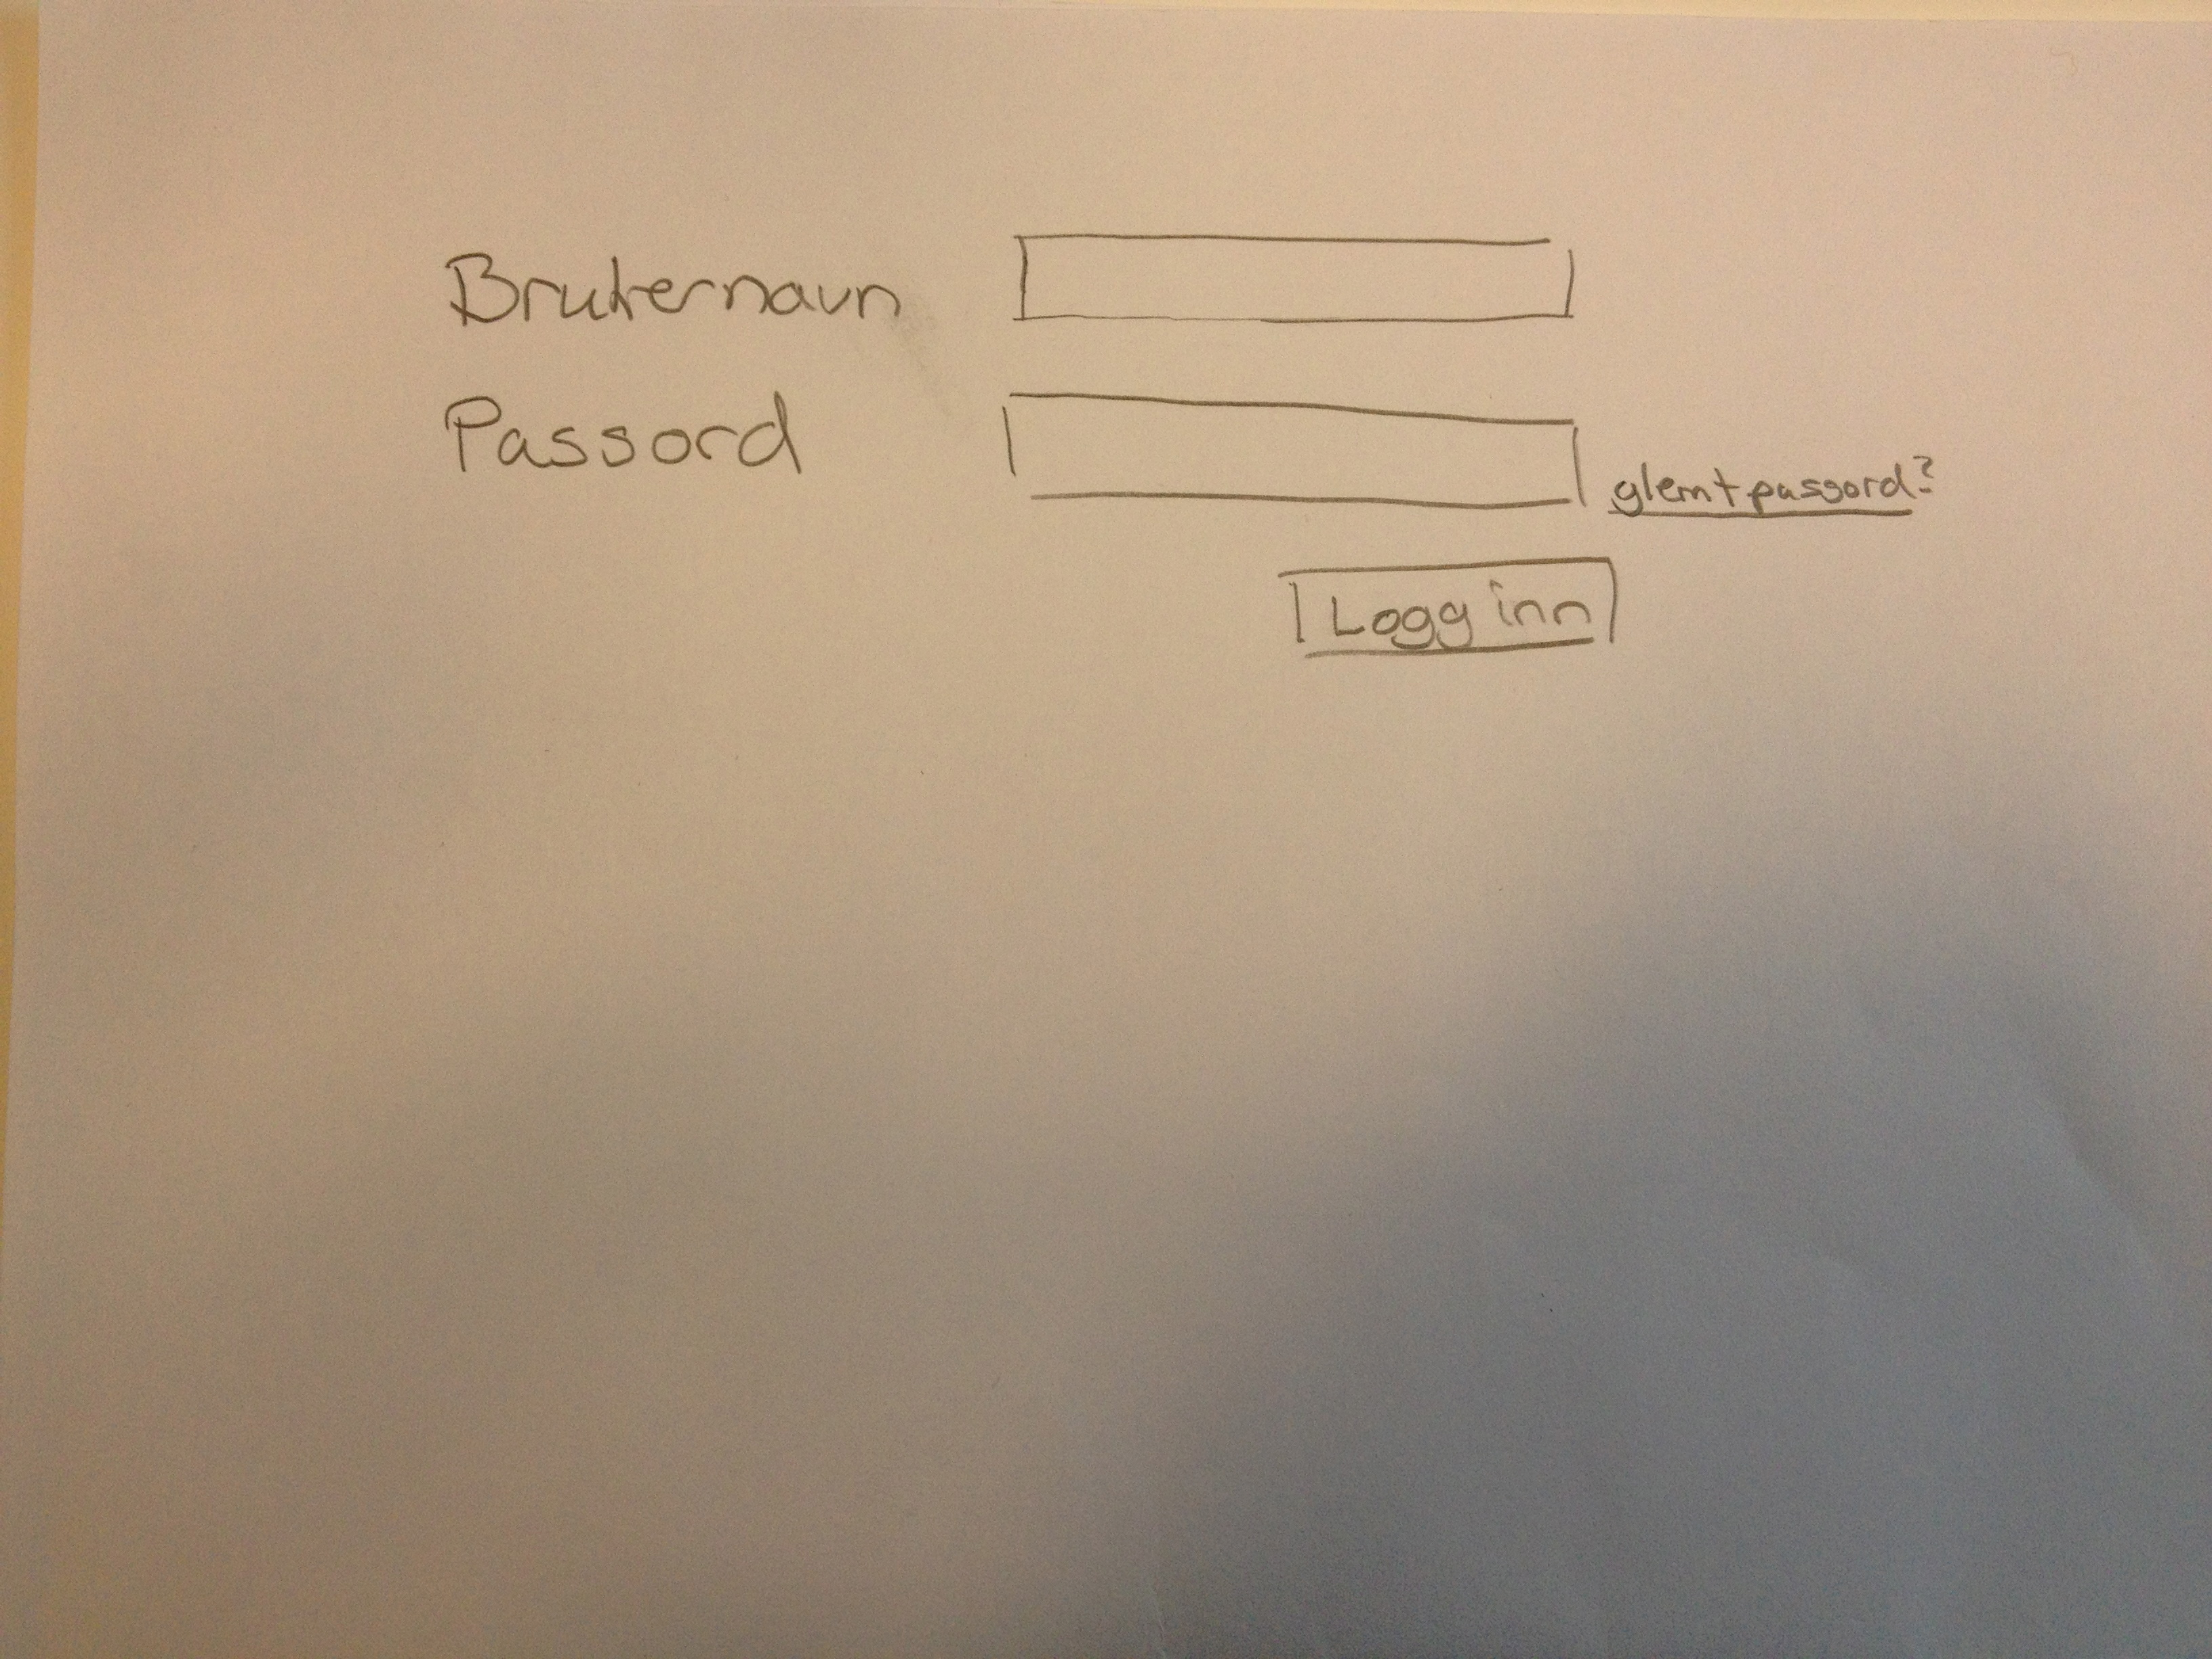
\includegraphics[width=90mm]{fig1.jpg}
\caption{Innloggings vindu}
\end{figure}
En helt enkelt innlogging skjerm der brukeren kan skrive brukernavn og passord. Vi kan også benytte “glemt passord” som tar oss til fig2. Dersom brukeren skriver feil navn eller passord, så vil det skrives ut: “feil passord og/eller brukernavn”. Dersom bruker skriver riktig informasjon, så vil han bli tatt til fig3.
\newpage

\subsection{Glemt passord}
\begin{figure}[ht!]
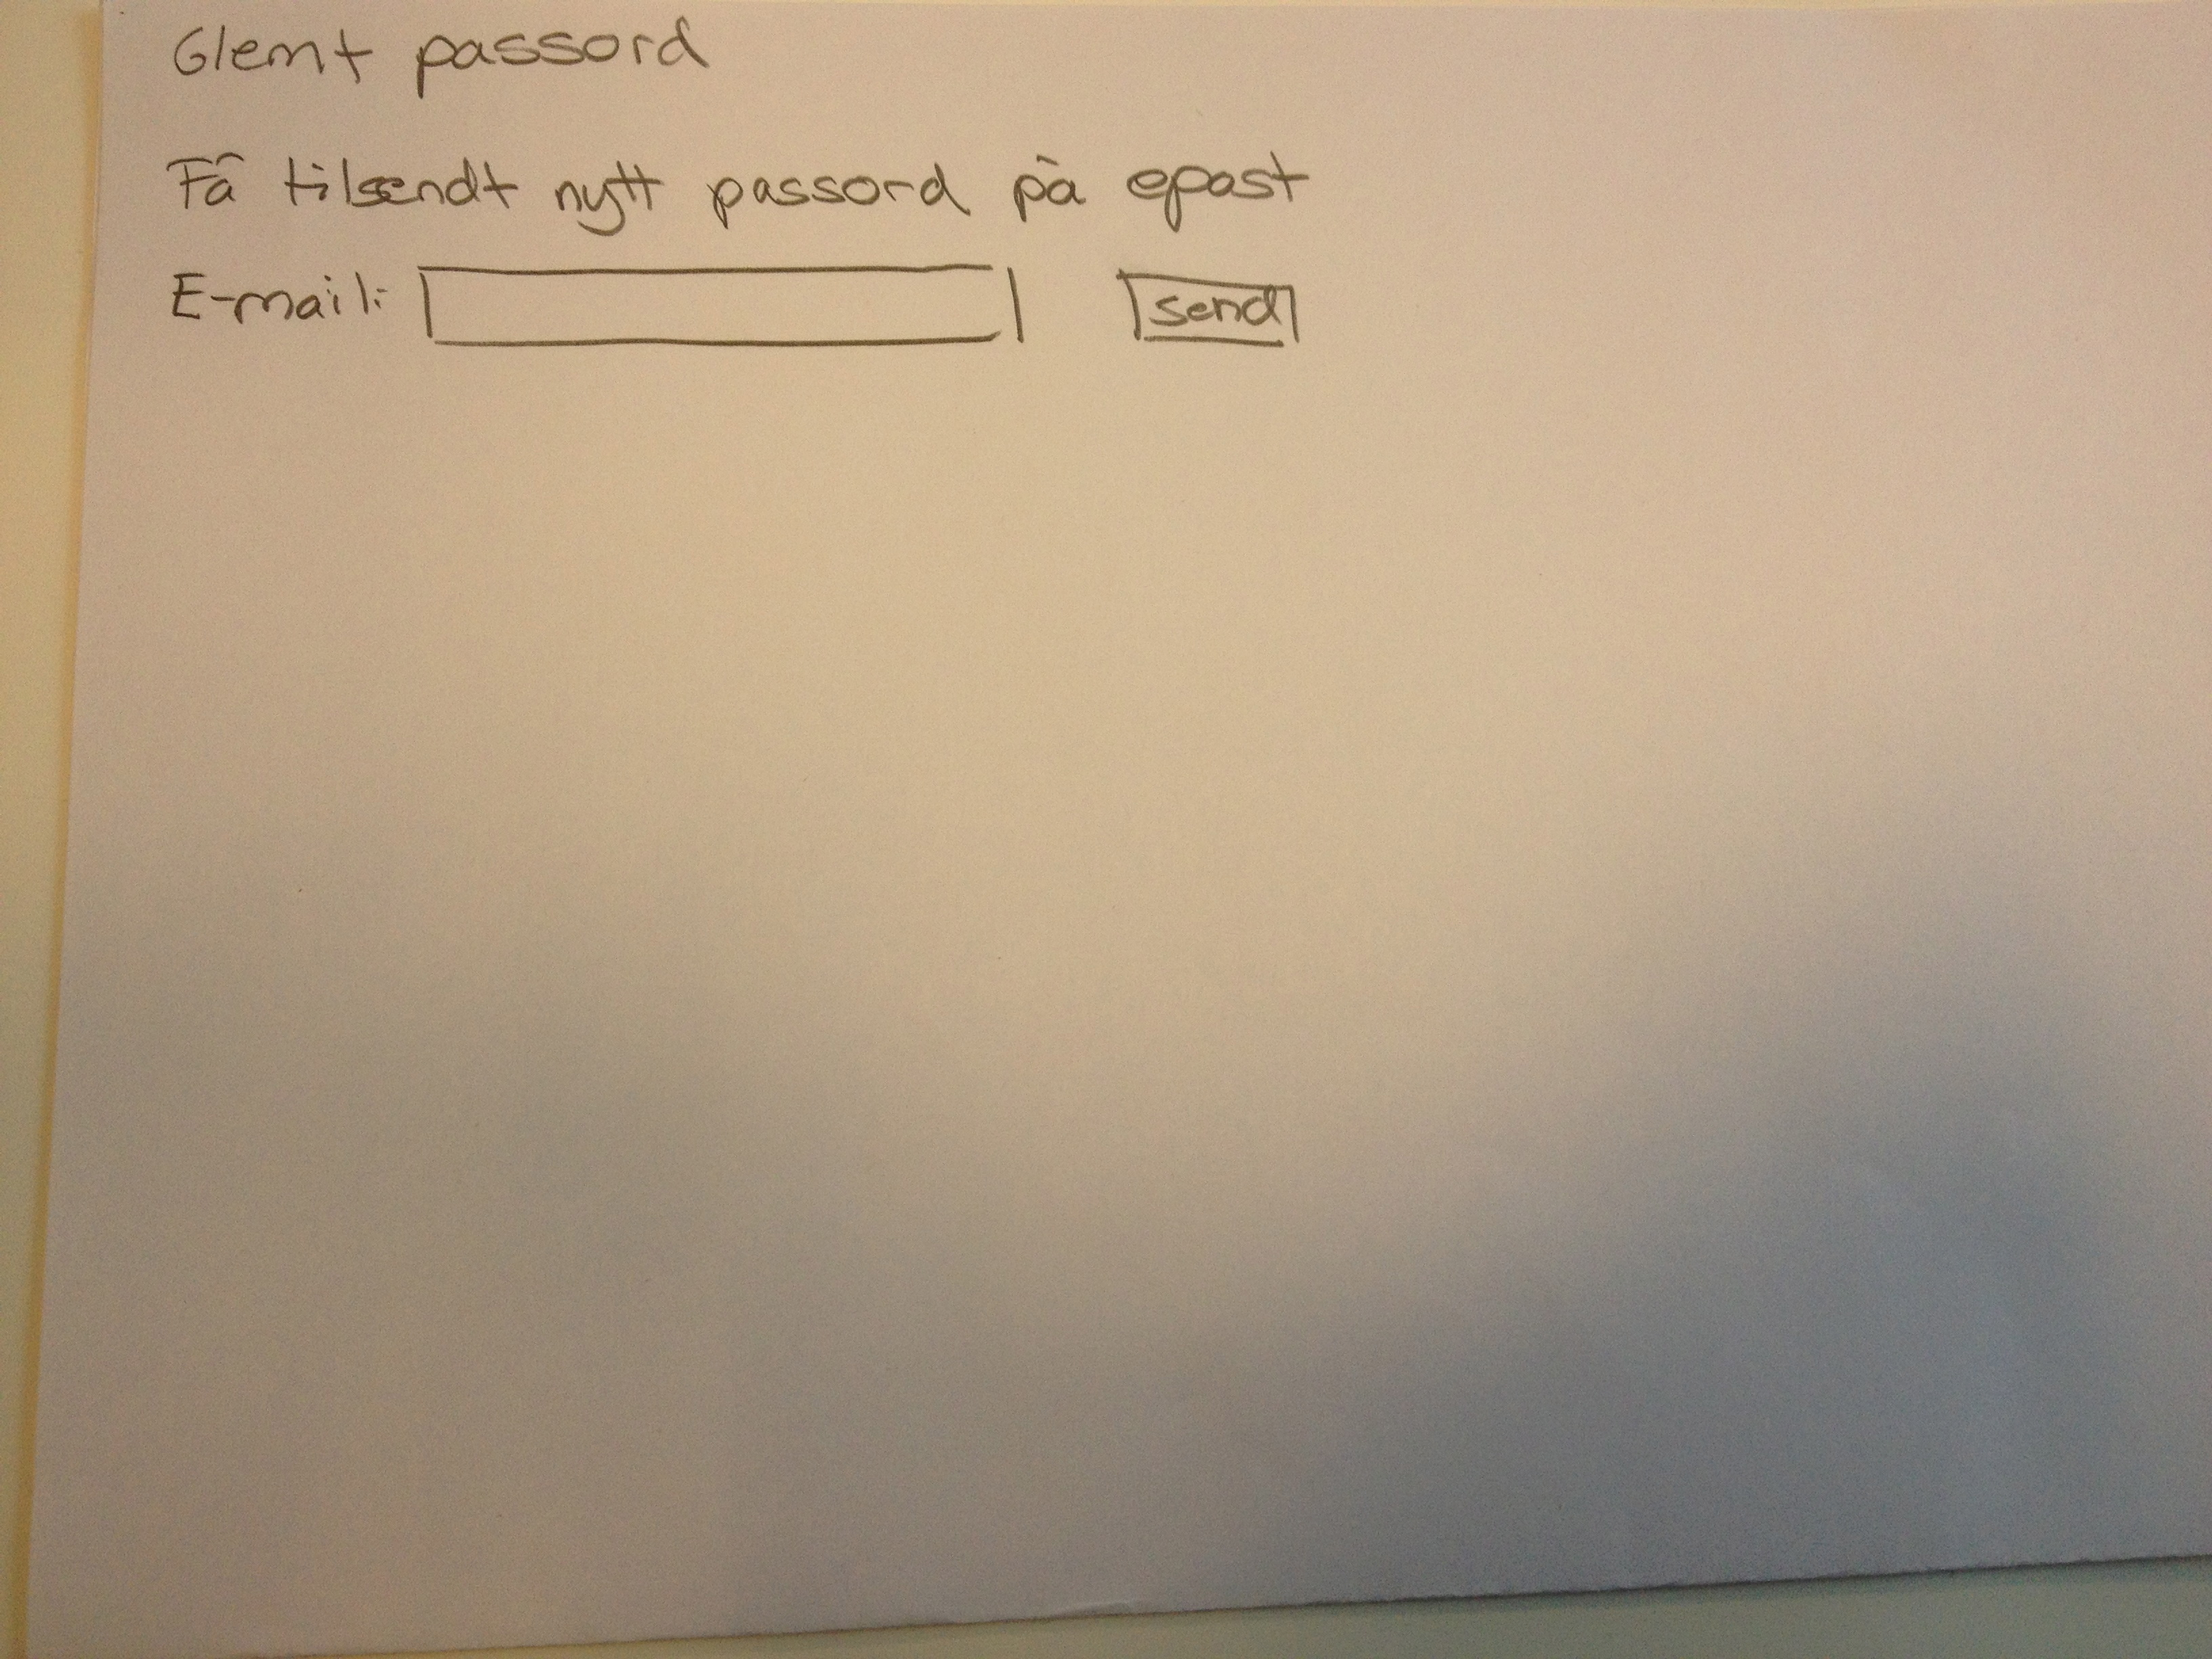
\includegraphics[width=90mm]{fig2.jpg}
\caption{glemt passord skjerm}
Et ny vindu som popper opp, her skriver man e-mail/brukernavn, avhengig av hva firma X bruker, så får de tilsendt sitt passord til sin e-mail.
\end{figure}

\newpage

\subsection{Kalendervisning}
\begin{figure}[ht!]
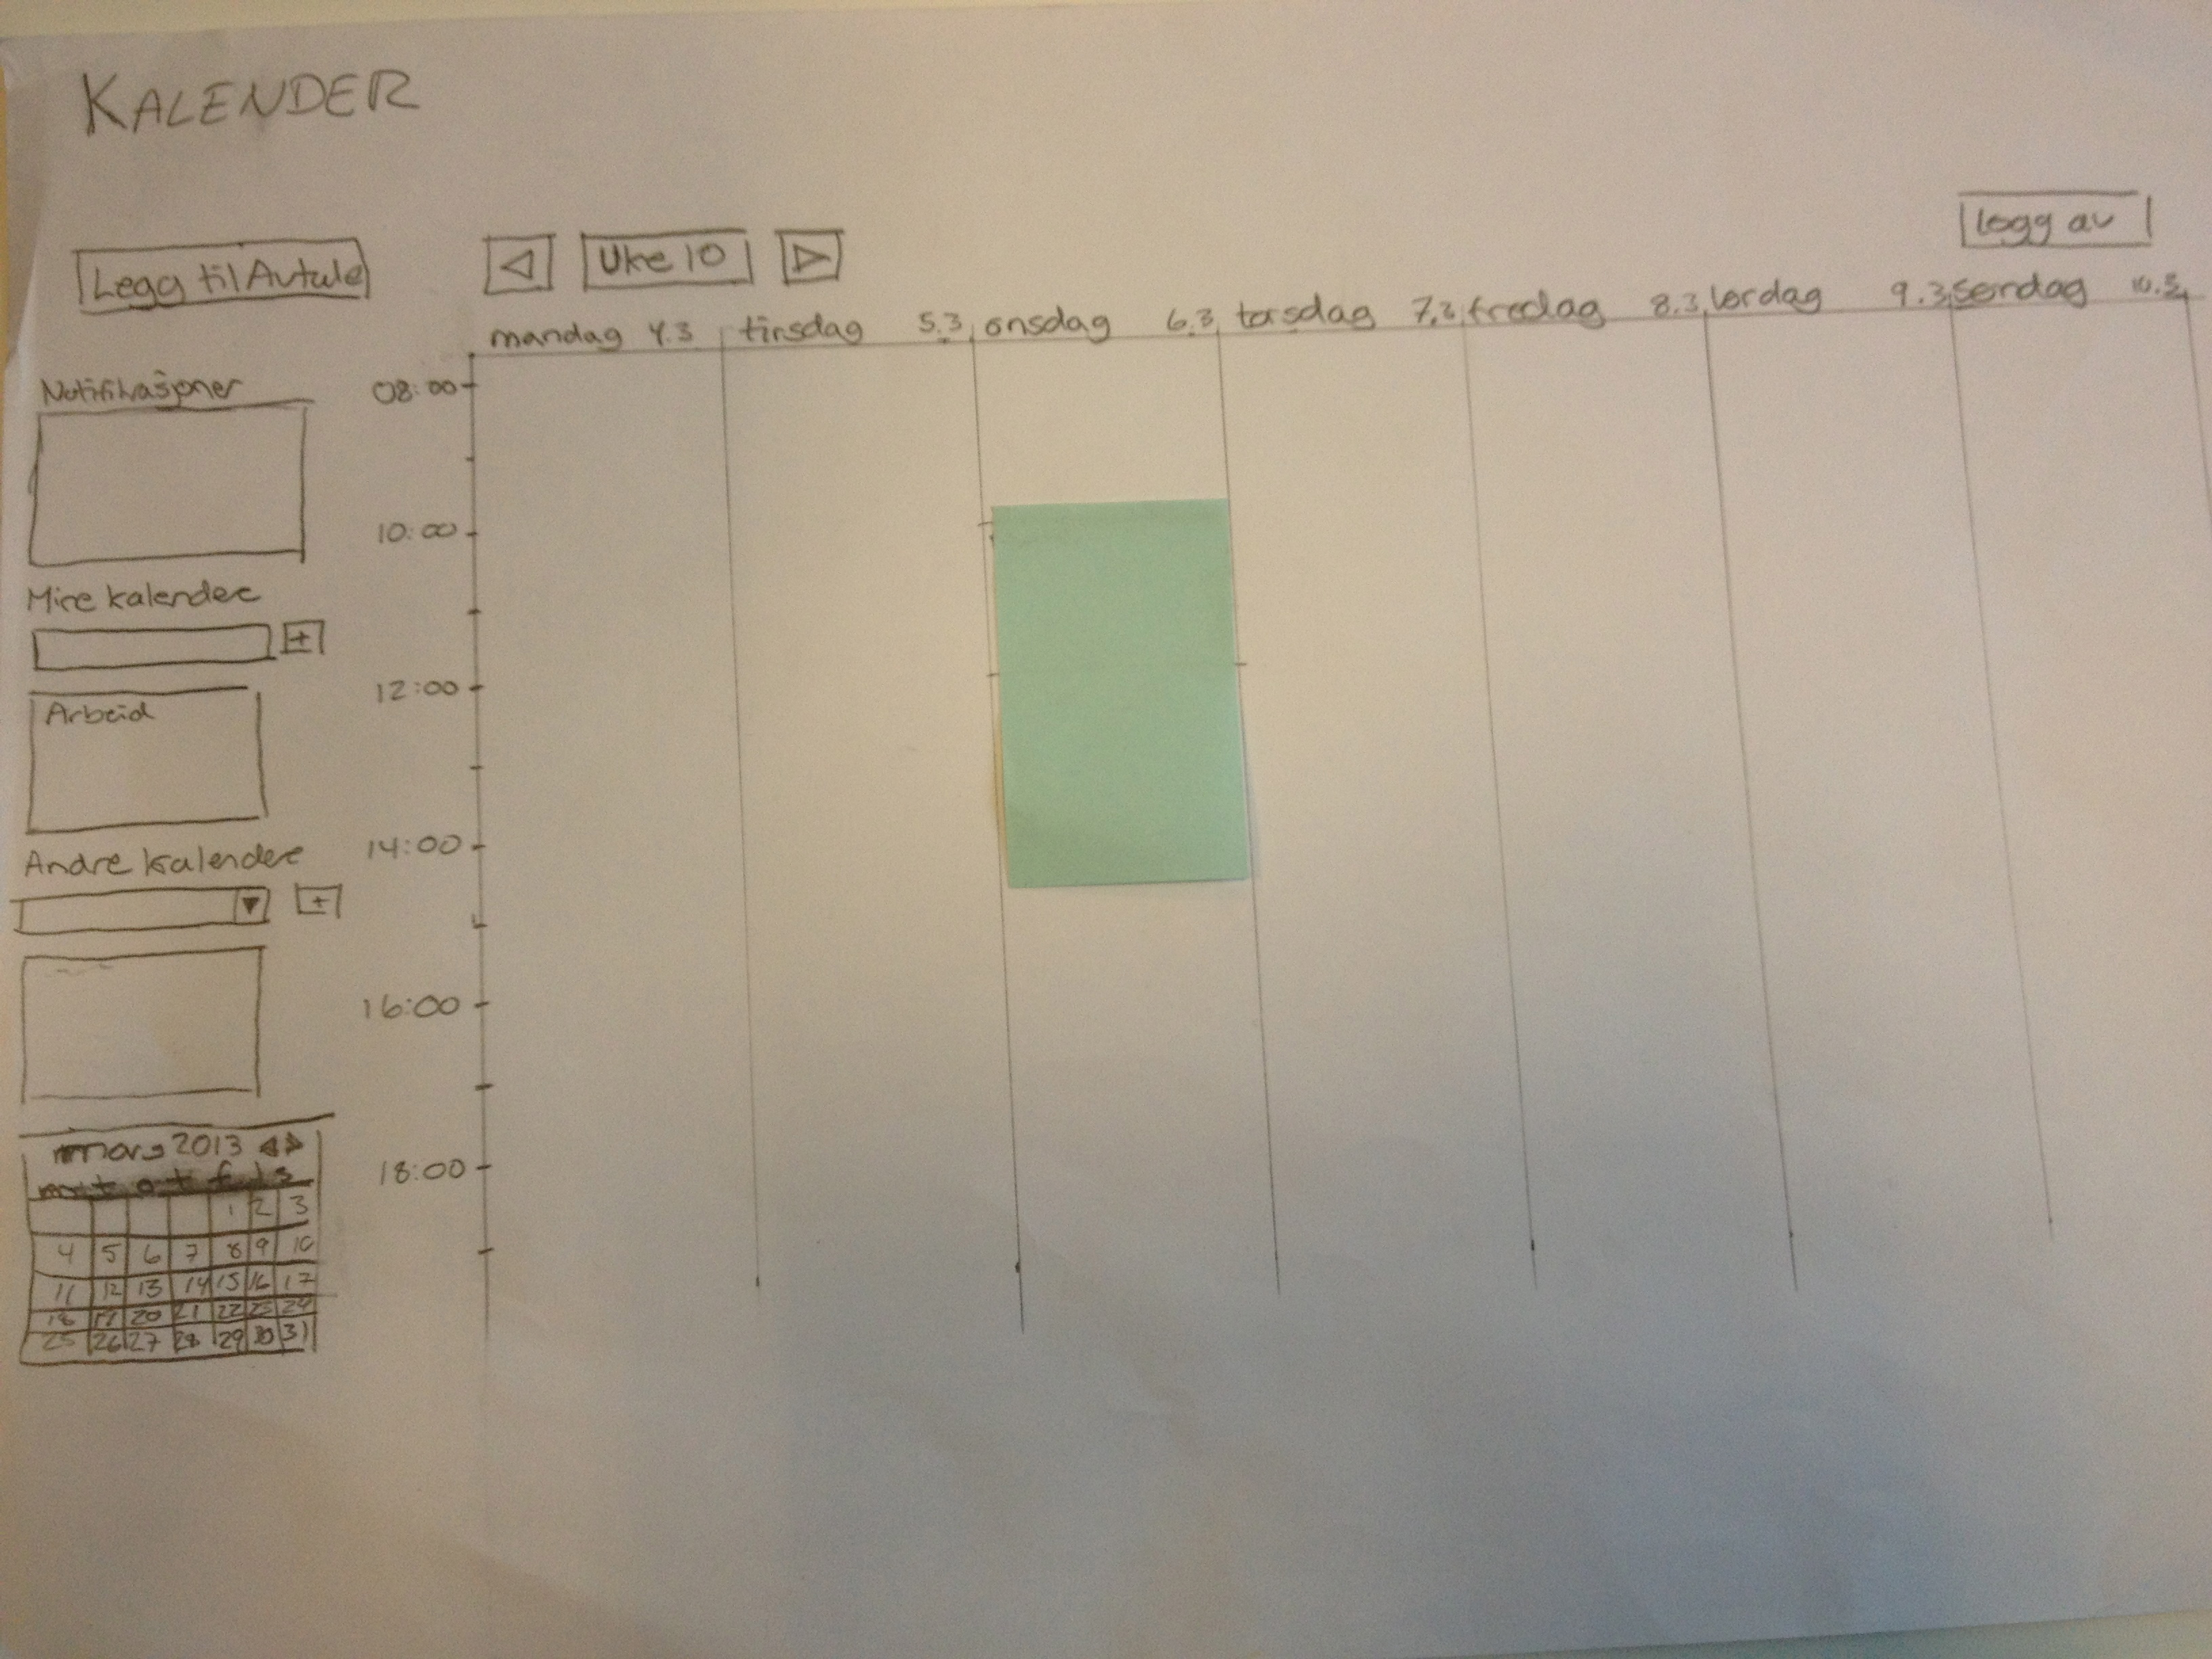
\includegraphics[width=100mm]{fig3.jpg}
\caption{Kalendervisning}
\end{figure}
Her er selve ukedagkalenderen. Man ser at på venstre side av figuren så har man flere valgmuligheter, blant annet notifikasjonsvindu. Man kan se forskjellige notifikasjoner til møter som brukeren ikke har svart på. Dersom man blir invitert til et møte, så dukker det opp en melding i vinduet, og man får muligheten til å trykke på den og fig7 dukker opp. 

Under der er det en liste av andre kalendere som brukeren kan lage selv. Man trykker på feltet og skriver hva man vil kalle kalenderen. Under der igjen så har vi de andre sine kalendere, vi tenkte at man skal kunne hente andre brukere sin kalender for å lettere kunne velge ett tidspunkt som passer for flere personer til et møte. Andre brukere sine kalendere er i forskjellige farger så man lettere kan skille dem fra hverandre. Vi har også en månedskalender under for å holde styr på ukene som kommer. Vi har valgt å ta med hvilket ukenummer det er nå, siden folk ofte benytter ukenummer, og mange andre kalendersystem ikke viser det. Øverst ser vi en knapp som heter “legg til avtale”, man trykker på den for å opprette en ny avtale og kommer da til fig4. Man kan også endre på hvilken uke kalenderen skal vise, det gjør man ved hjelp av pilene ved siden av ukenummeret. Øverst i høyre hjørne er det en logg av knapp, som logger brukeren av systemet.

\newpage

\subsection{Oppretting av møte}
\begin{figure}[ht!]
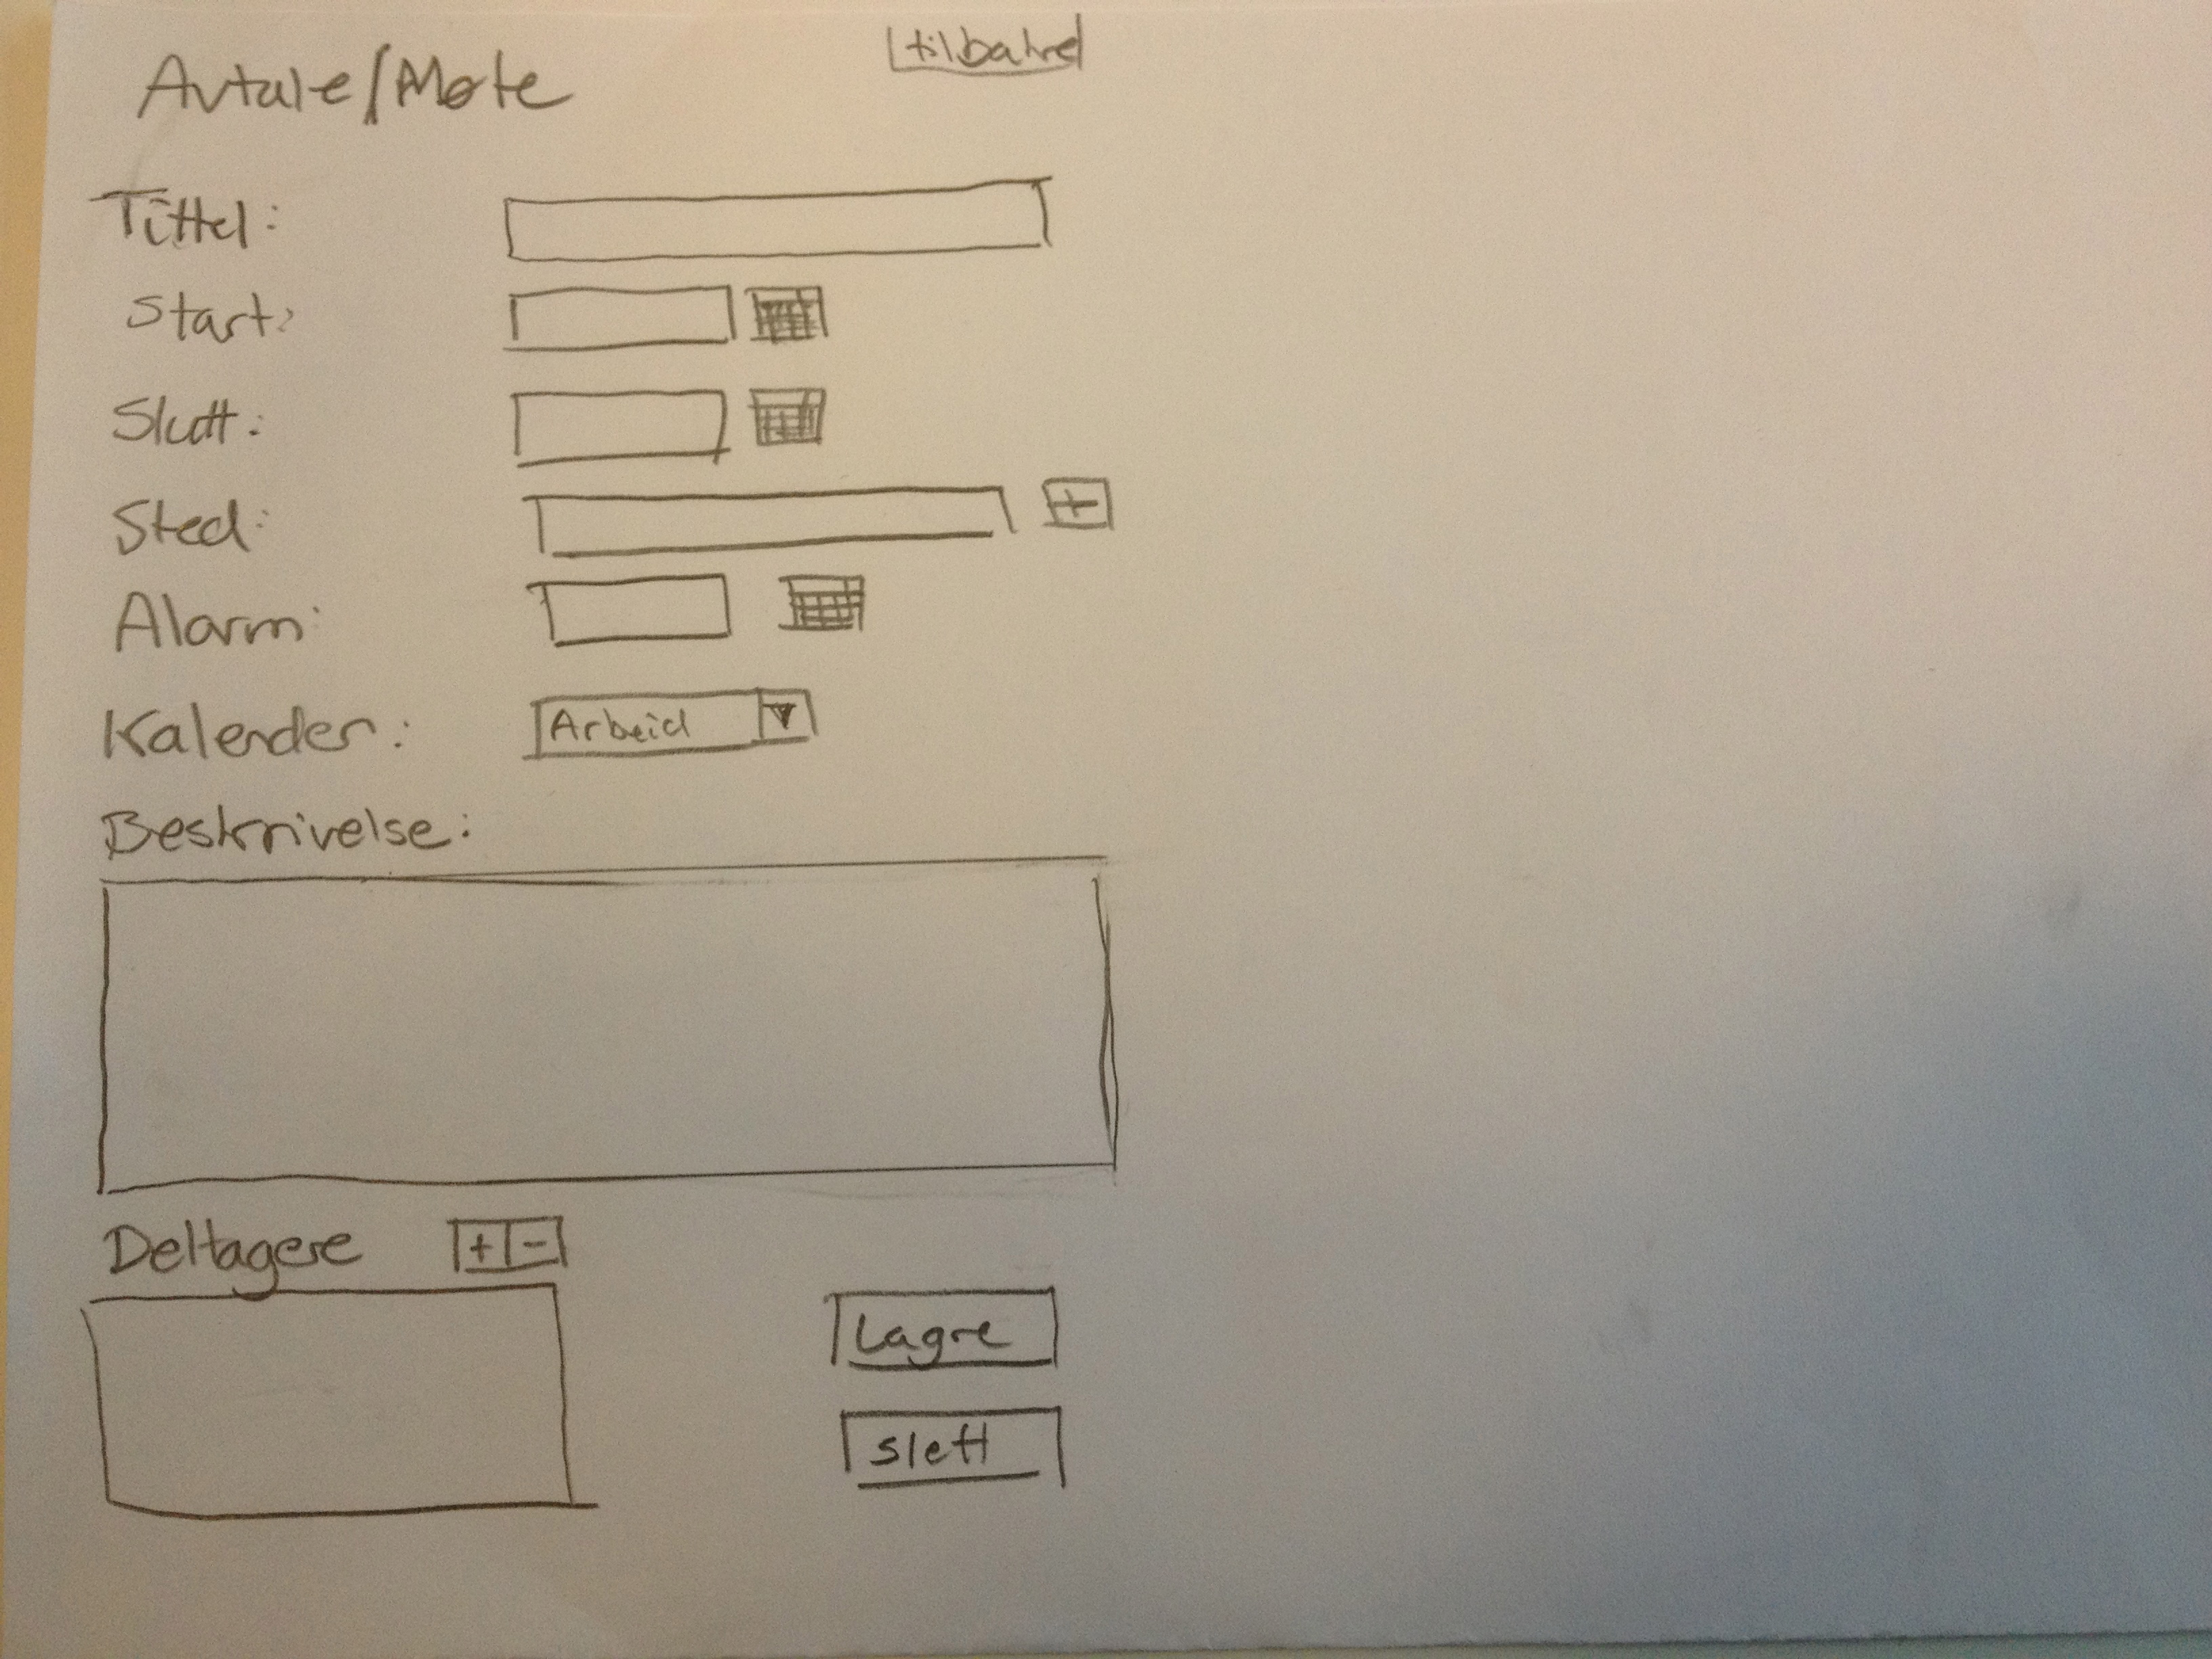
\includegraphics[width=90mm]{fig4.jpg}
\caption{Laging av møteinnkalling og avtale}
Her kan man opprette avtale, alle feltene skal kunne fylles ut, og når man trykker på kalenderikonet ved siden av tid så dukker det opp en liten månedskalender der man kan velge hvilken dag man vil ha. I den lille kalenderen så er det også et lite felt der man kan skrive det bestemte tidspunktet. Man kan i feltet for sted skrive inn et valgfritt sted eller reservere et møterom ved å trykke på “+” knappen. Fig5 popper da opp.
Under beskrivelse kan man skrive inn en kort beskrivelse av møte/avtalen. For å legge til deltagere trykker man på  “+” knappen og fig 6 kommer opp. Mens hvis man trykker på en deltager og trykker “-”  vil den valgte personen slettes fra deltagerlisten. Så kan man enten lagre eller slette avtalen med knappene. 
\end{figure}

\newpage

\subsection{Rommbestilling}
\begin{figure}[ht!]
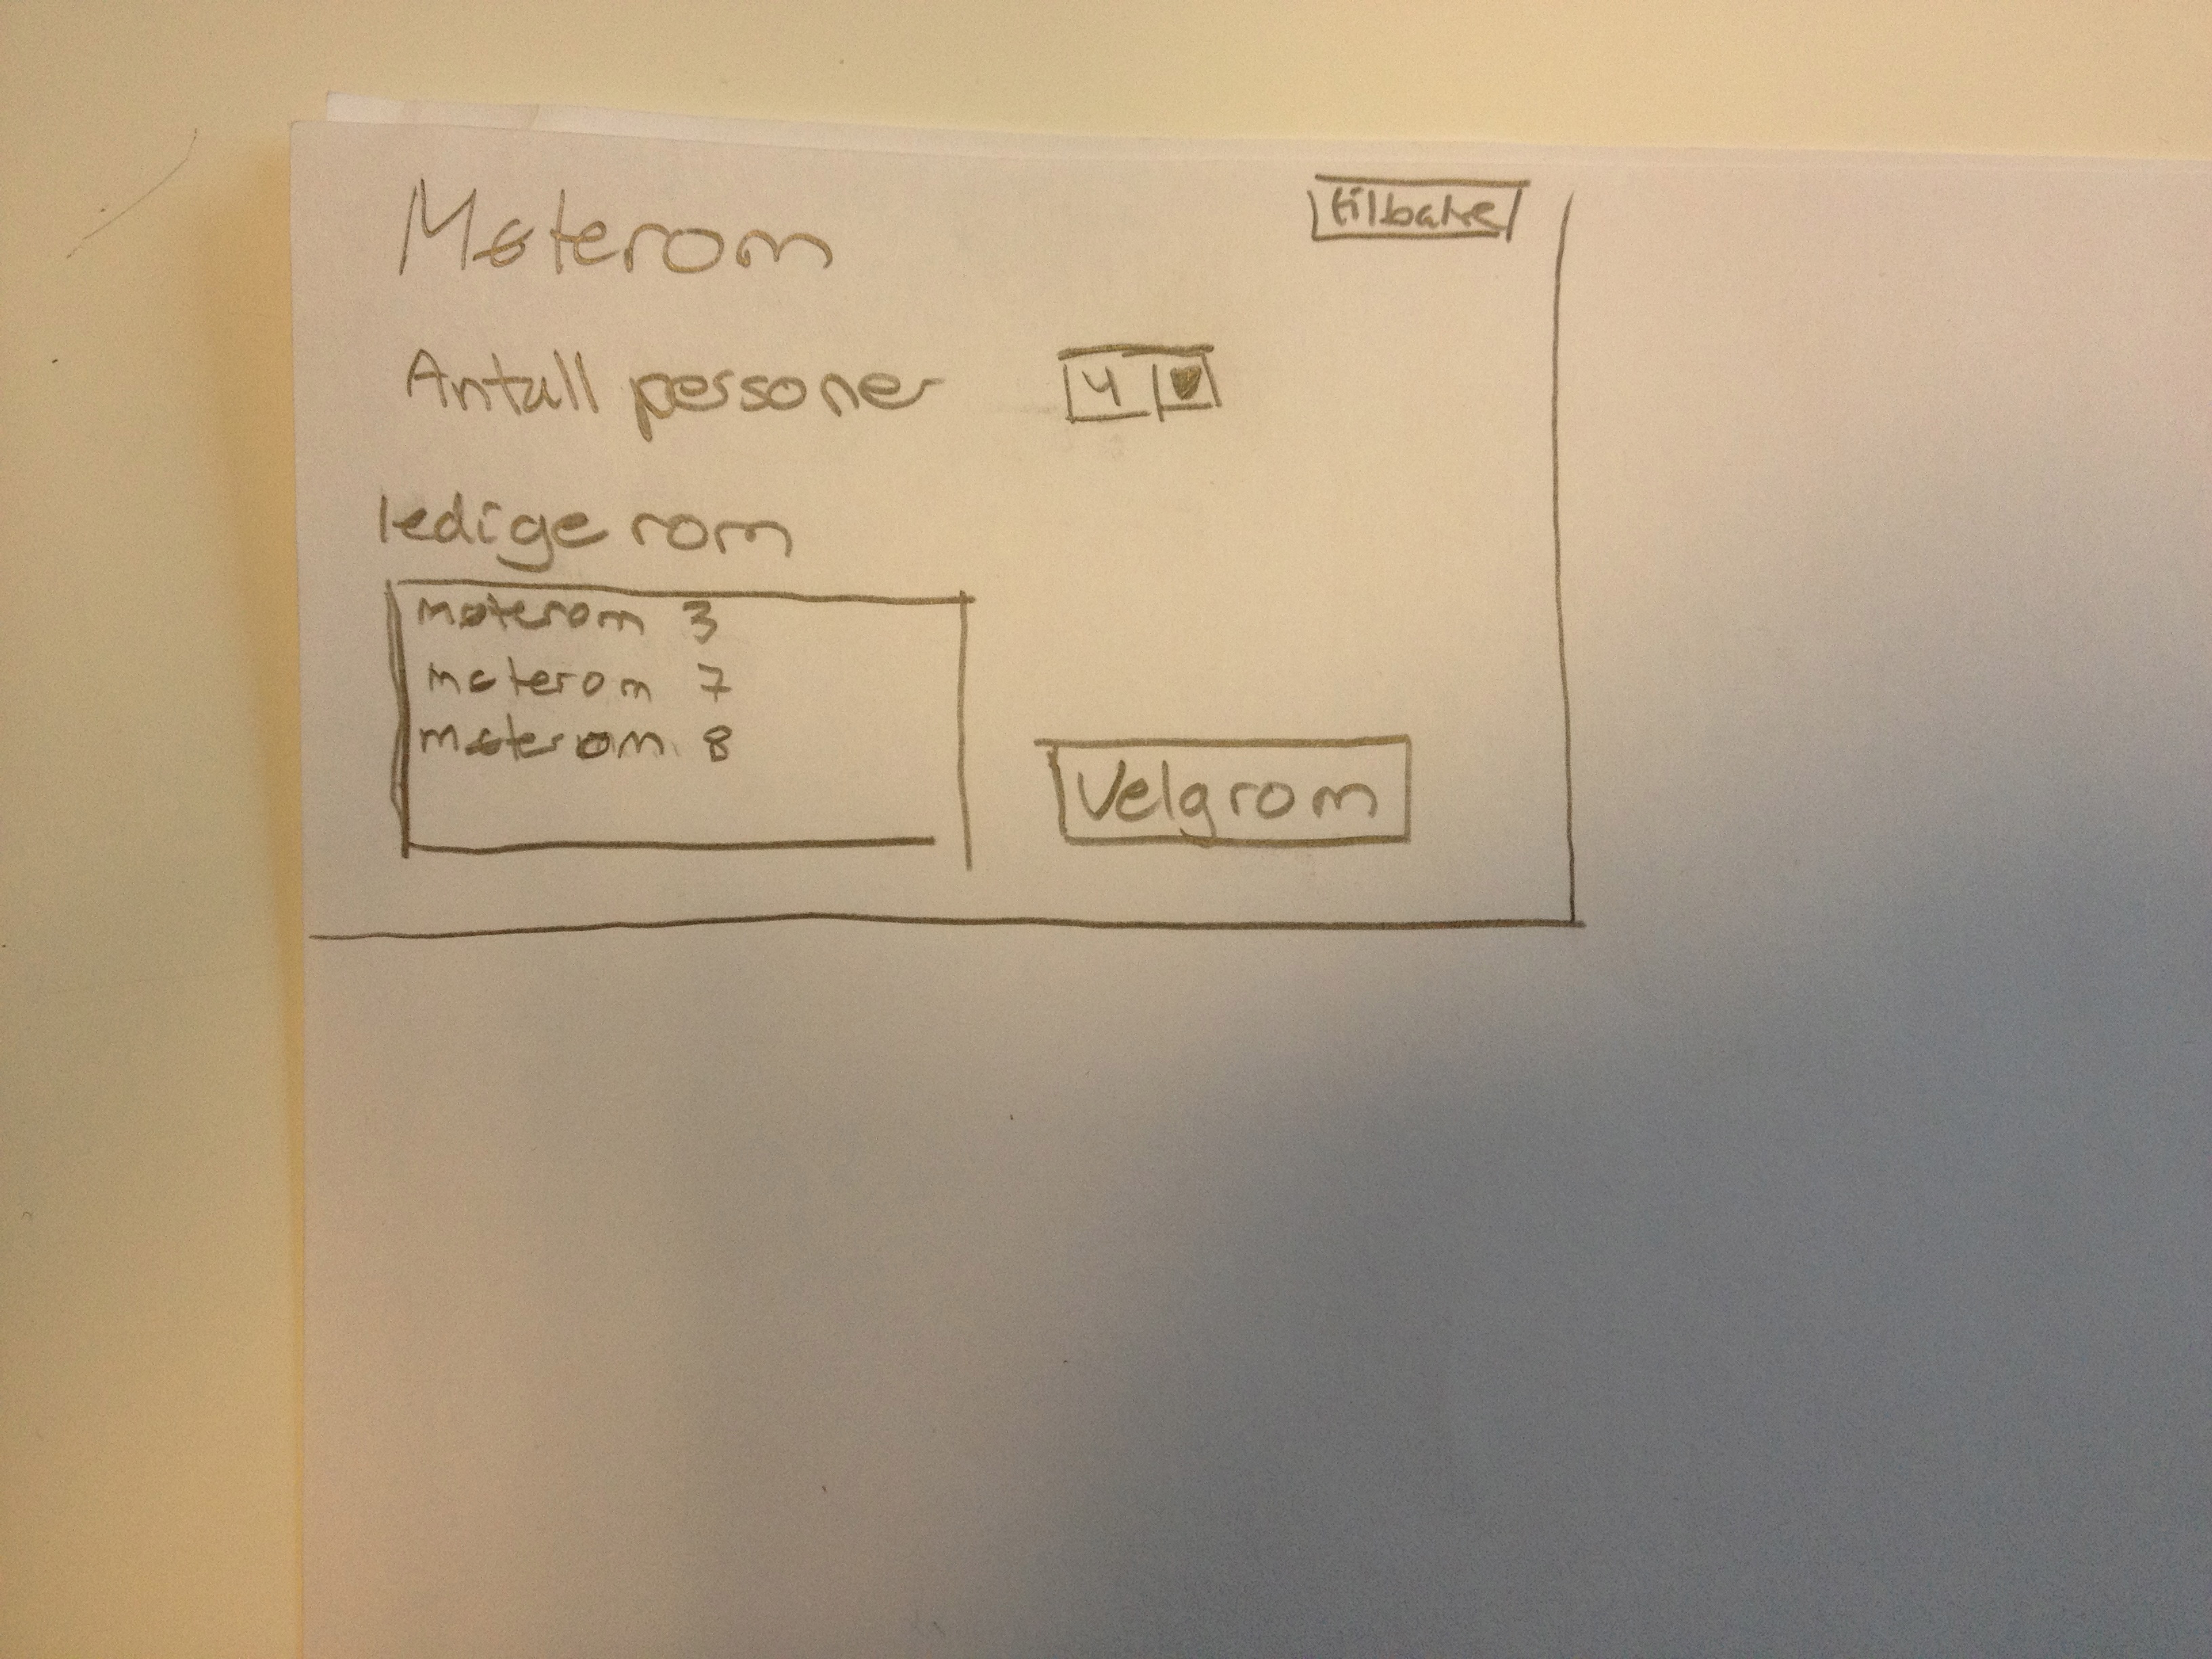
\includegraphics[width=90mm]{fig5.jpg}
\caption{Bestilling av rom}
Her har man en scroll-bar som man bruker til å velge antall personer, og en liste med ledige rom i tidsperioden avtalen er satt til. Man bekrefter valgene sine ved å trykke på “velg rom”. Dersom man trykker på “tilbake”, så vil man bli tatt tilbake til fig 3.
\end{figure}

\newpage


\subsection{Legge til deltager}
\begin{figure}[ht!]
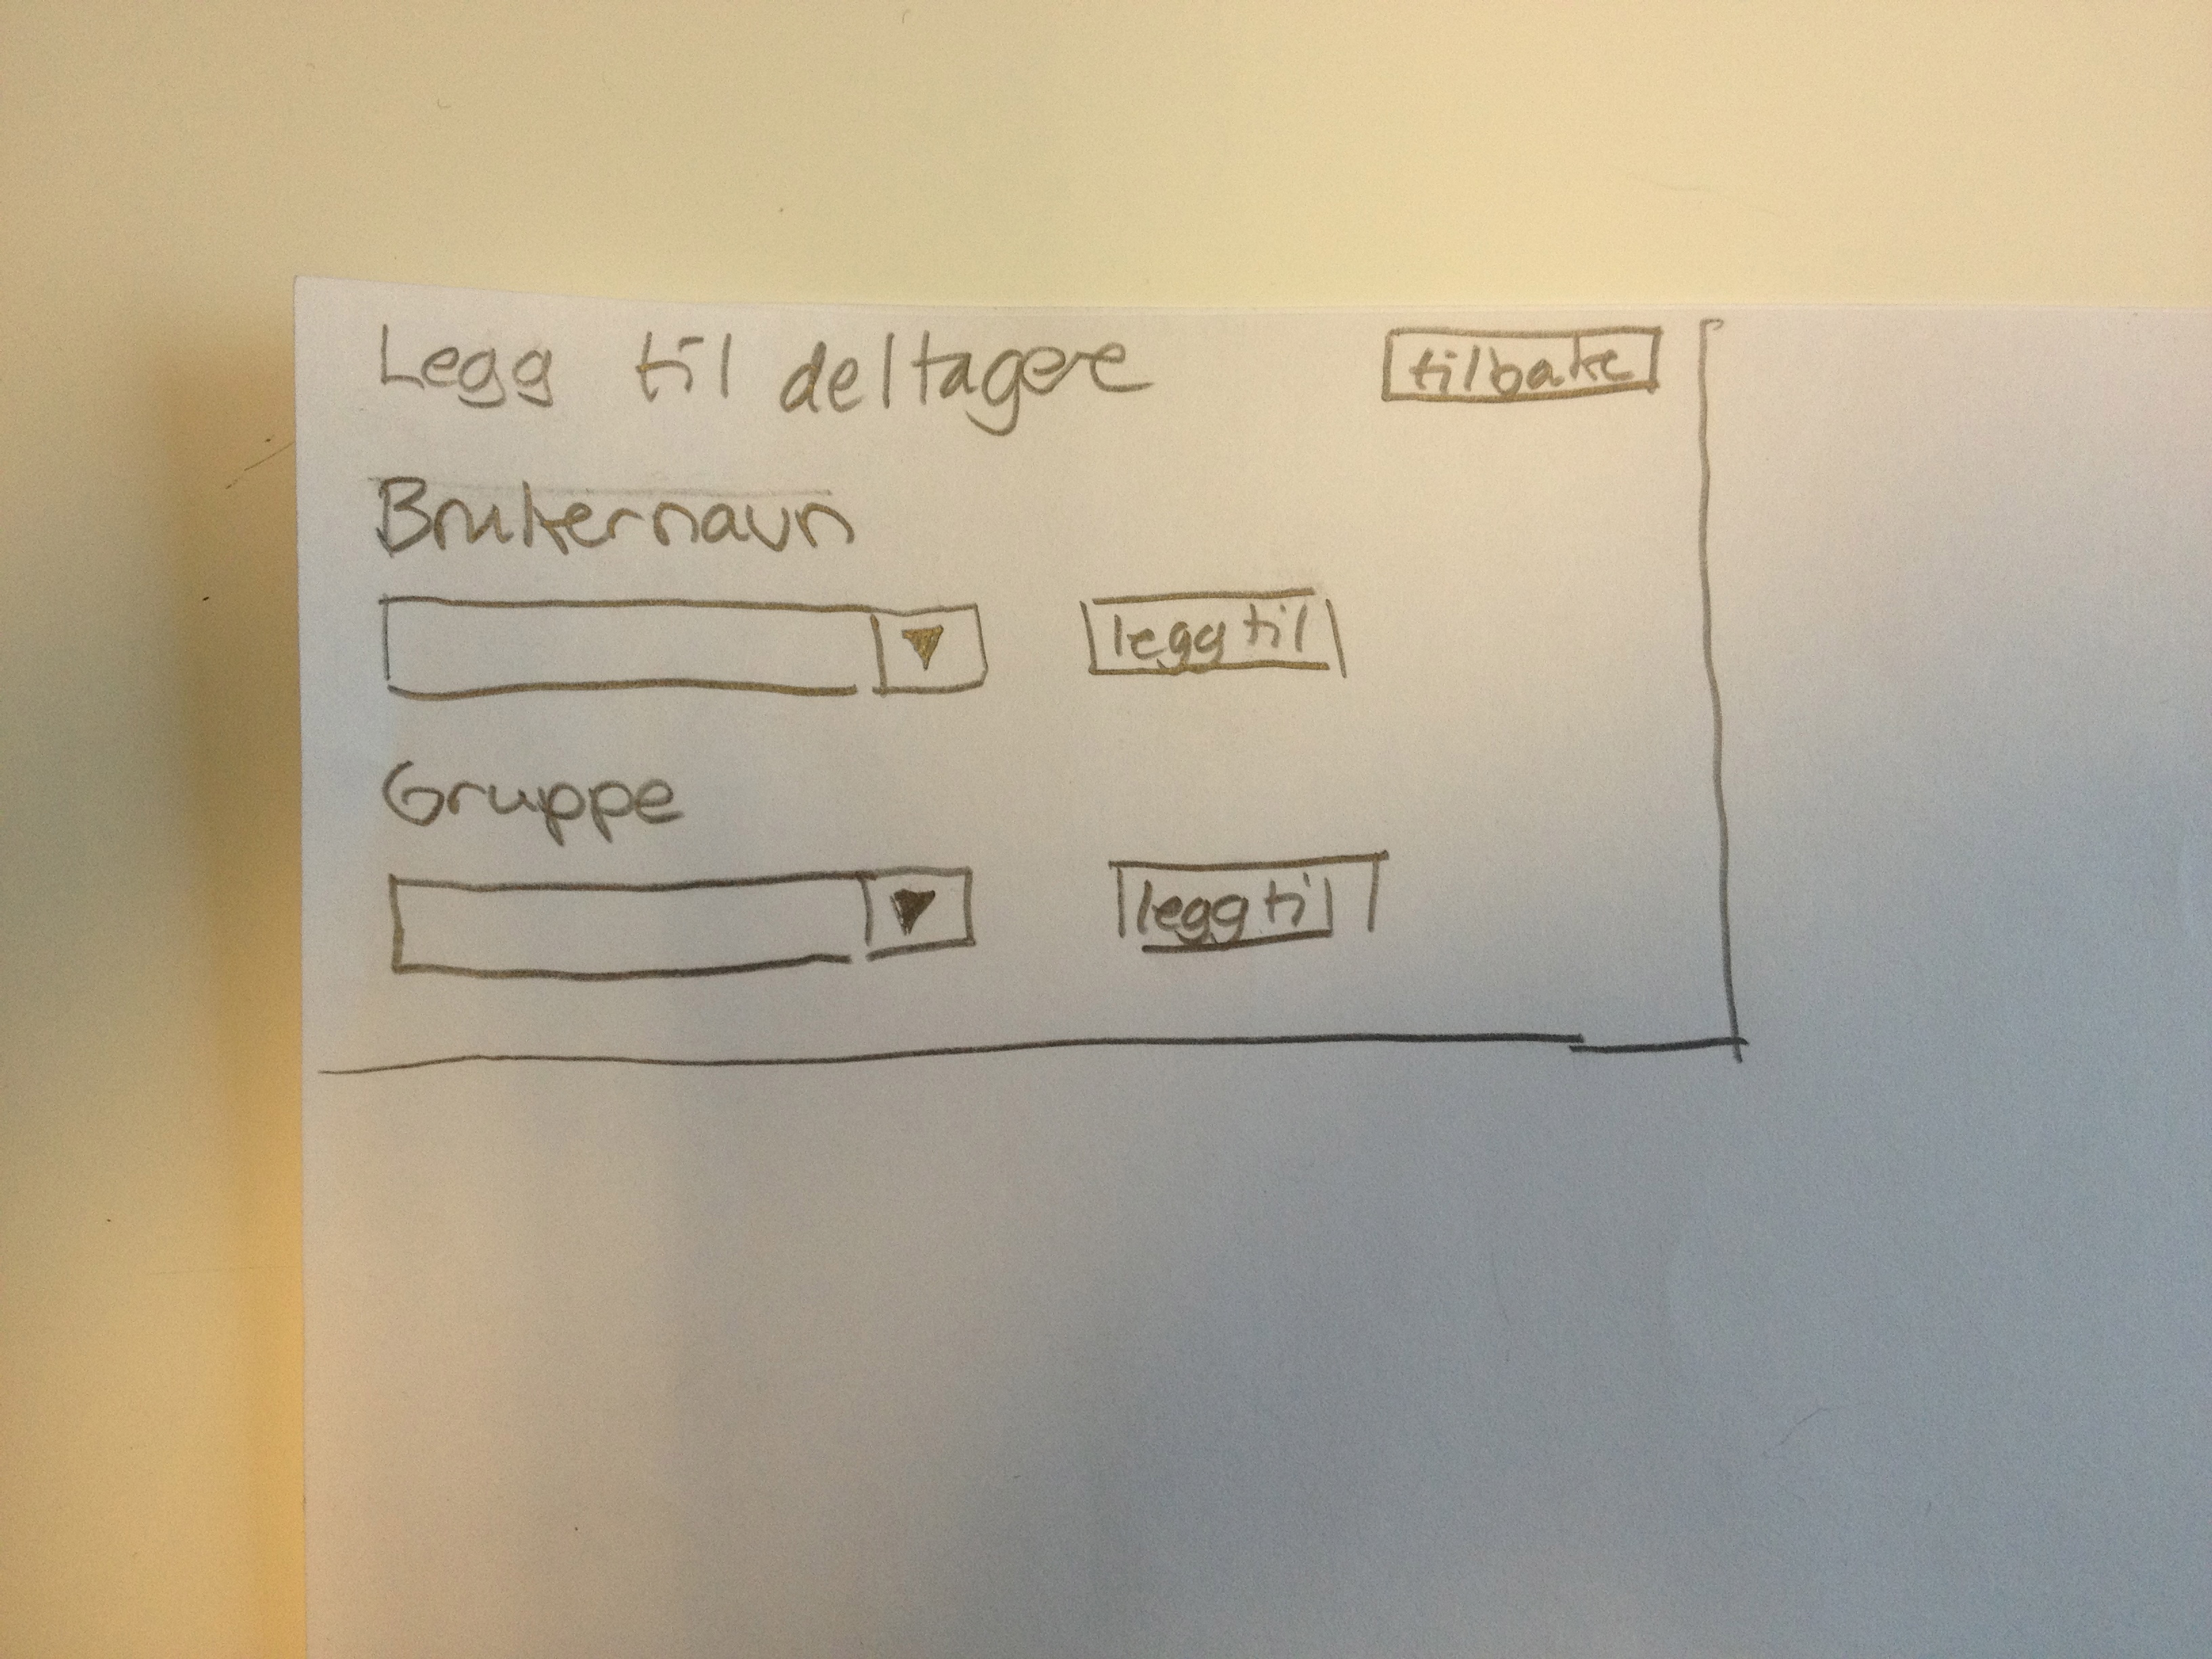
\includegraphics[width=90mm]{fig6.jpg}
\caption{ Legge til Deltager}
Her er det to felt, det ene feltet kan man skrive brukernavnet til hver bruker, pilen er for å illustrere at når man begynner å skrive navnet til en deltager, så kommer forslagene under i form av en liste. Ett av kravene var også at det skal være mulig å legge til en gruppe med personer. Dette gjøres på samme måte som når man legger til en bruker, bare ved at man skriver inn gruppenavn. Da vil alle brukerne som er lagt til i gruppen bli invitert som enkeltpersoner.
\end{figure}

\newpage
\subsection{Avtalevisning}
\begin{figure}[ht!]
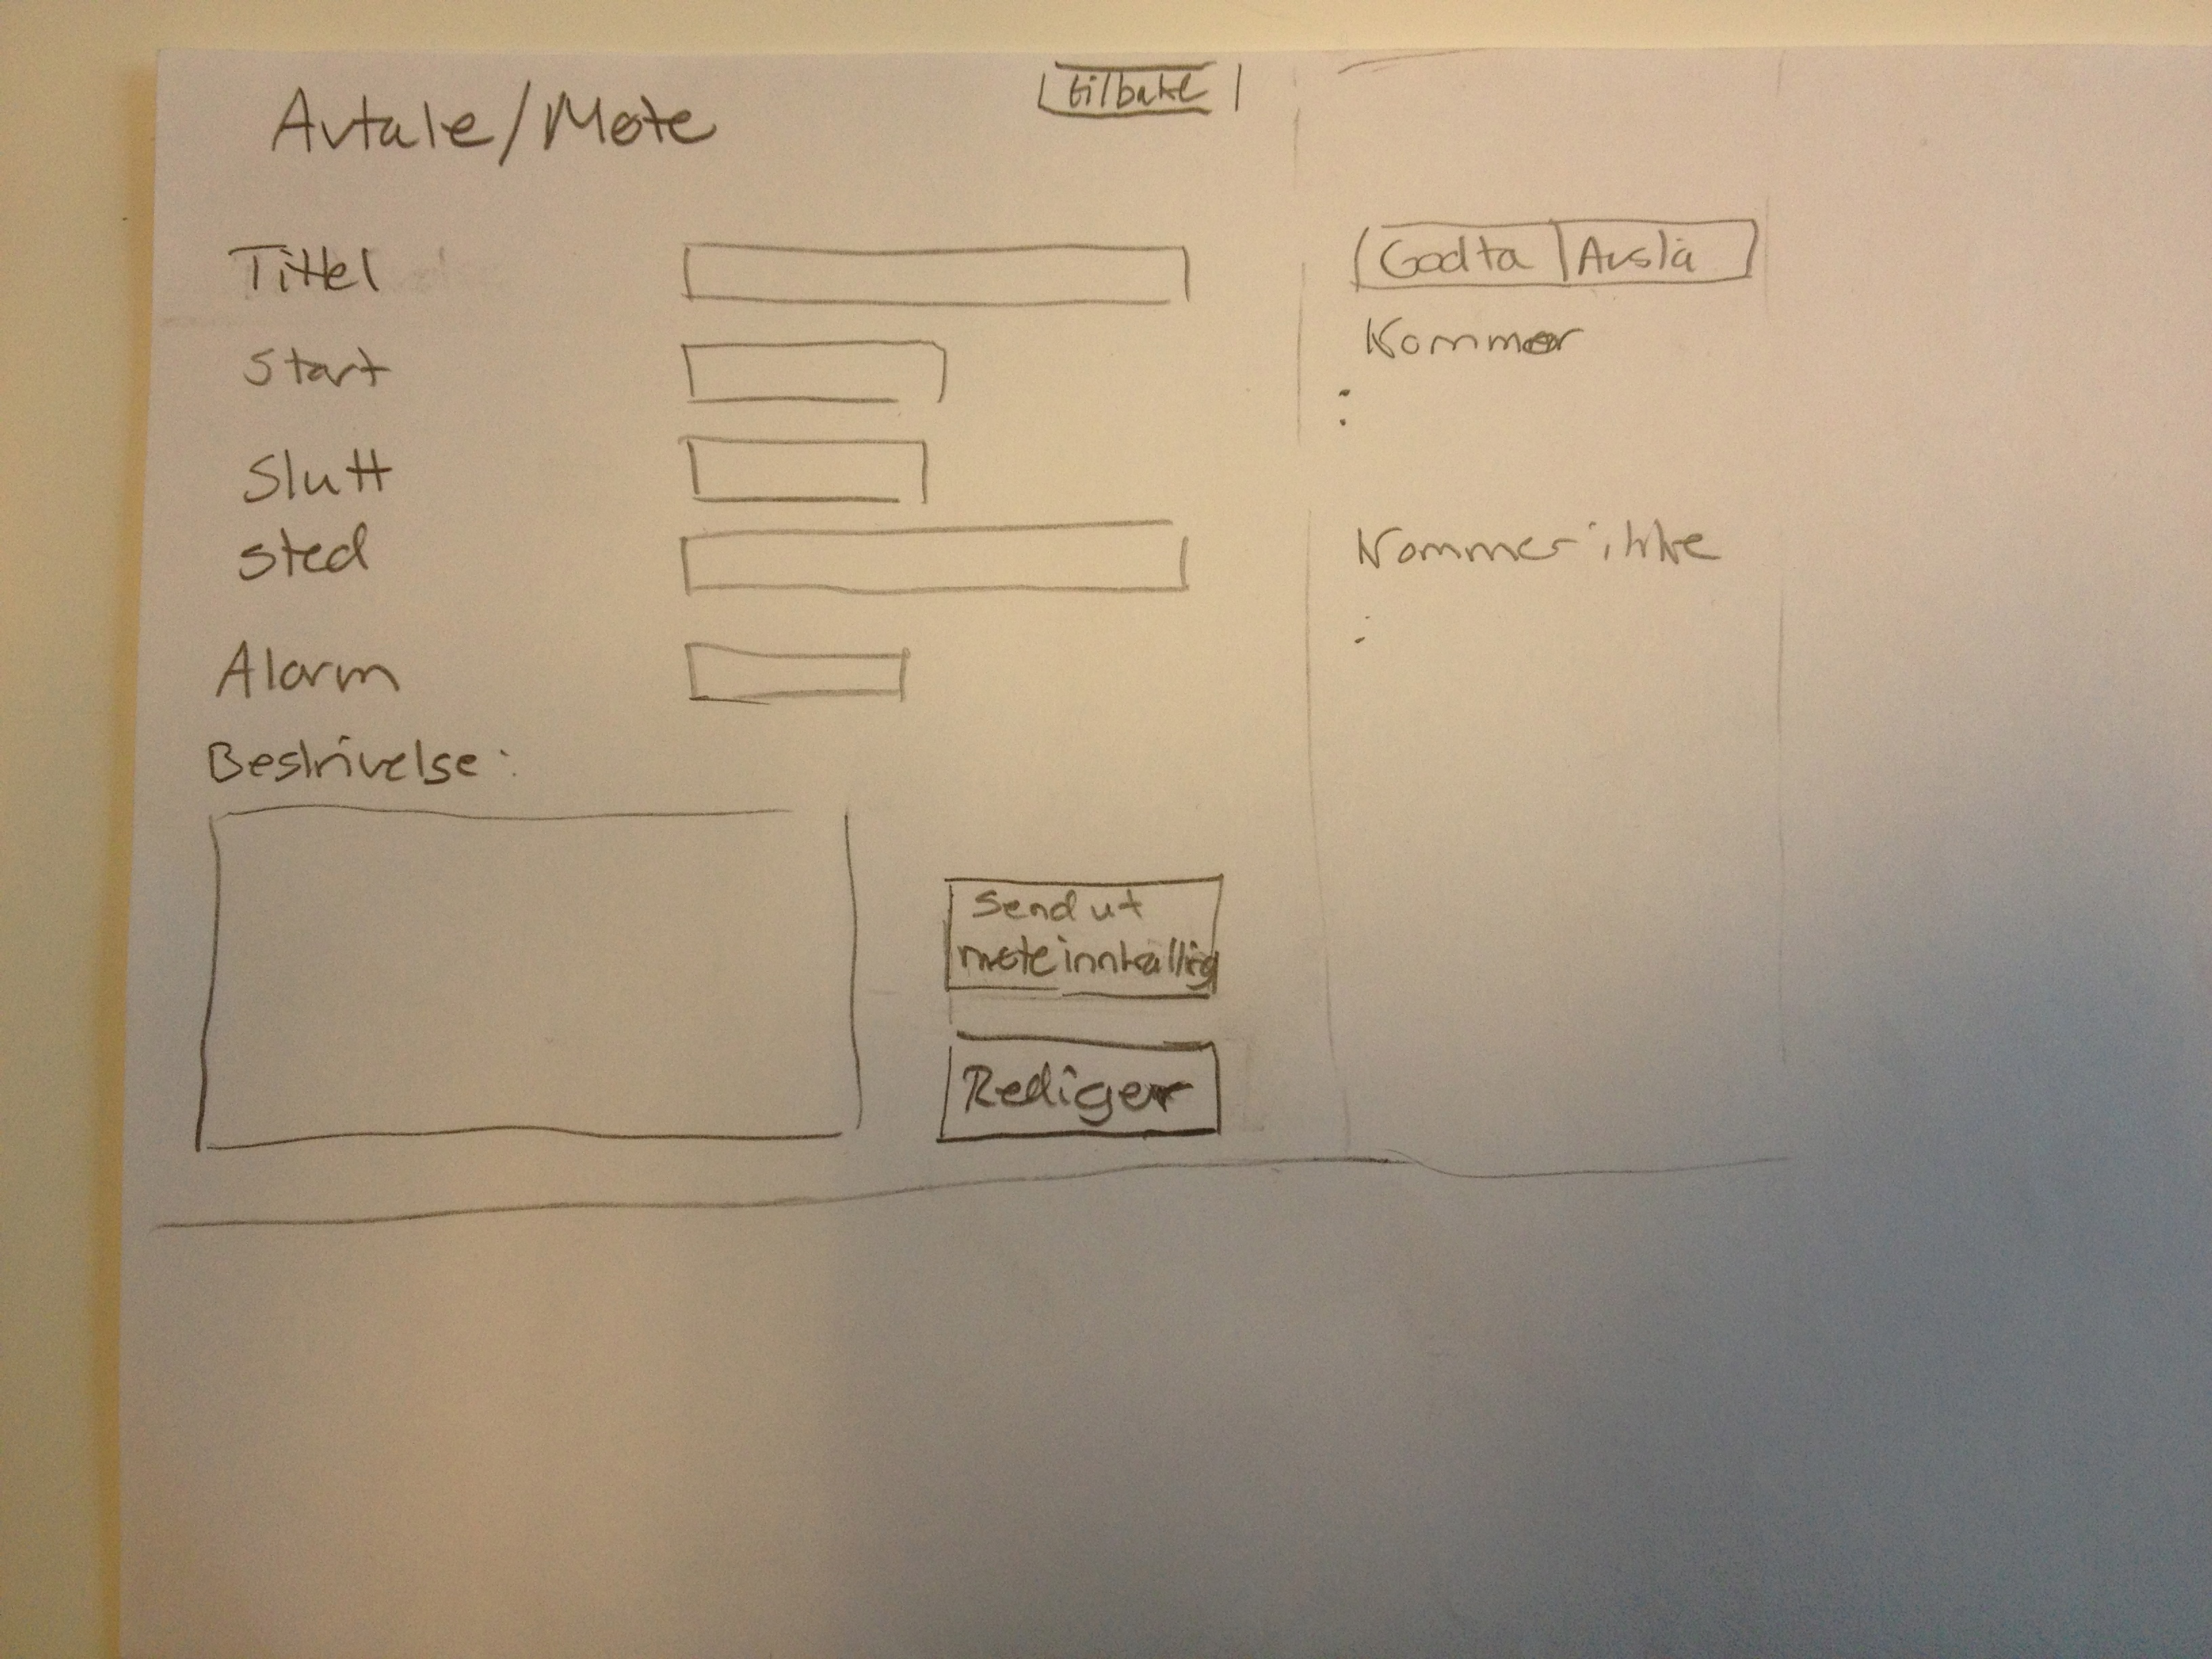
\includegraphics[width=90mm]{fig7.jpg}
\caption{Avtalevisning}
Her vises alle opplysninger angående avtalen, feltene kan ikke endres. Dersom man er møtelederen(personen som opprettet møte), har man også mulighet til å sende ut møteinnkalling. Når man har trykket på send notifikasjon, så vil alle deltagere få oppdatering når møtet blir endret. Er man møteleder har man muligheten til å endre på møte, og knappen “rediger” vil ta deg tilbake til fig4. Til høyre for figuren så ser man to mulige knapper, godta og avslå, dersom man velger en av dem, så blir den muligheten grået ut. Man kommer da på listen under, over hvem som kommer og hvem som ikke kommer. “tilbake”-knappen vil ta deg tilbake til fig3.
\end{figure}

%slutt seksjon med newpage
\newpage 

\begin{figure}
\section{State-diagram}

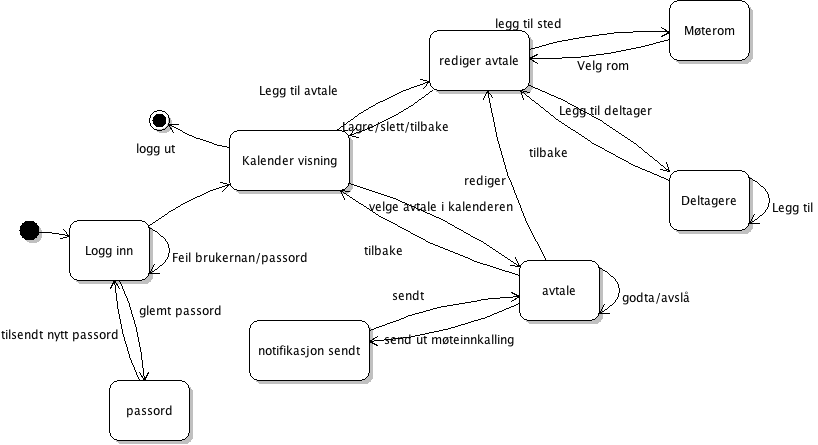
\includegraphics[width=150mm]{MMIstatediagram.png}
\caption{Statediagram}
\end{figure}
\newpage

\section{Oppgavelisten}
Testpersonen vår fikk litt mer frihet, de fikk et par konkrete oppgaver som de skal klare, blant annet: 
\begin{itemize}
	\item Logg inn
	\item Lage en avtale
	\item Sette en tidspunkt til en avtale
	\item Legge til to personer
	\item Fjerne en person fra en avtale
	\item Velge et rom til en avtale
	\item Slette en eksisterende avtale.	
\end{itemize}
Brukeren kunne selv velge i hvilken rekkefølge de ville gjøre oppgavene i. Disse kravene er enklere nedbrutt versjon av scenarioene som vi fikk tildelt. 
%\\ %tvinger frem en ny linje, kan kombineres til flere \\\\ => to nye linjer
%forferdelig at det er disse to tegna som brukes, men sånn er det

\newpage

\section{Gjennomføring}
Etter at vi hadde avtalt tid med grp 39, gikk vi til dem for å gjennomføre testen. Vi fikk en person fra deres gruppe til å teste vår papirprototype, og noterte ned eventuelle vanskeligheter og problemer som testpersonen fikk. De begynte med å først logge inn, deretter gikk de gjennom forskjellige oppgaver og scenario som de lagde selv. 

Etter at testen ble gjennomført fikk vi tilbakemeldinger fra alle i deres gruppe. Siden gruppen deres satt og så på under utførelsen, så tenkte vi at det virker litt meningsløst å få resten av gruppen til å gå gjennom hele testen på nytt igjen.

%inkludért seksjon, hva vi burde bruke
%\input{filnavn.tex}
%input setter inn teksten som er i filnavn.tex, og vi kan dermed style i dette dokumentet

%referanseliste
\section{SUS resultater}
3+3+3+4+2.5+4+4+4+3+4=34.5
34.5*2.5=86.25
det gir oss en sum på 86.25/100

Ut ifra poengfordelingen så ser vi at vårt design virker lett forståelig og lett å komme i gang med. Siden vårt design tar inspirasjon fra kjente paradigmer innen kalenderapplikasjoner, og folk flest har kjennskap til det, så krever det nesten ingen opplæring av systemet.
\newpage
\includepdf{SUS_skjema1.pdf}

\section{Uklarheter}
Brukeren hadde et par uklarheter under testen. Testpersonen hadde litt vanskeligheter med å forstå “+” og “-” ikonene der man legger til en person. Vi fikk også beskjed om at det virker litt merkelig at “+” og “-” symbolene var veldig nært hverandre, og de så ut som om de var av samme  gruppe, men ga forskjellige reaksjoner, den ene må man velge en person, mens den andre popper opp et nytt vindu der man kan legge til en ny person.  Feltet der man skriver var litt for smått (hvordan formatet på tiden skal være var også litt uklart). 

Det virket også som folk misforstod hvordan man sletter en avtale. Vårt orginale design var at brukeren må redigere avtalen og der kan man velge å slette den, men testpersonen valgte å trykke avslå på sin egen avtale og forventet at sin egen avtale blir slettet. Det er noe som kanskje burde vært tydeligere eller så kan vi implementere at når man avslår sitt eget møte/avtale så slettes den automatisk. 

\section{Endringer}
Endringene som vi gjorde med systemet blir da at når man trykker på “+”, så kommer det et ekstra vindu oppå det originale kalendervinduet. I motsetning til det originale designet der man kommer til et helt nytt vindu. Kan eventuelt gjøre det mer intuitivt eller skille de to symbolene mer fra hverandre, for eksempel ved bruk av tekst. Problemet er at det virker mer intuitivt med de symbolene. vi kommer til å implementere slik at når gruppelederen avslår sin egen avtale på fig7, så vil avtalen/møte bli slettet.

\section{Eventuelle forbedring til prototypetesten}
Vi kunne ha fått flere personer fra deres gruppe til å teste papirprototypen, slik at vi fikk flere ulike kilder på eventuelle forbedringer. Det vil også gi oss et mer generelt syn på kalendersystemet vårt, i motsetning til nå som vi bare har en referanseperson. Under testen så satt hele deres gruppe og observerte testen. Vi burde ha tatt ut enkeltpersoner slik at vi kan bruke flere av deres gruppemedlemmer som testperson. Tiltross for at de ikke påvirket testen, så observerte de hvordan systemet var og dermed var det ikke noe vits i å be flere gå gjennom testen. 

\newpage
\listoffigures

\end{document}

